
% !TEX root = DesignDocument.tex

\chapter{Design  and Implementation}
This section is used to describe the design details for each of the major components 
in the system.    Note that this chapter is critical for all tracks.  Research tracks would do experimental design here where other tracks would include the engineering design aspects.    This section is not brief and requires the necessary detail that 
can be used by the reader to truly understand the architecture and implementation 
details without having to dig into the code.    Sample algorithm:  Algorithm~\ref{alg1}.  This algorithm environment is automatically placed - meaning it floats.   You don't have to worry about placement or numbering.  

\begin{algorithm} [tbh]                     % enter the algorithm environment
\caption{Calculate $y = x^n$}          % give the algorithm a caption
\label{alg1}                           % and a label for \ref{} commands later in the document
\begin{algorithmic}                    % enter the algorithmic environment
    \REQUIRE $n \geq 0 \vee x \neq 0$
    \ENSURE $y = x^n$
    \STATE $y \Leftarrow 1$
    \IF{$n < 0$}
        \STATE $X \Leftarrow 1 / x$
        \STATE $N \Leftarrow -n$
    \ELSE
        \STATE $X \Leftarrow x$
        \STATE $N \Leftarrow n$
    \ENDIF
    \WHILE{$N \neq 0$}
        \IF{$N$ is even}
            \STATE $X \Leftarrow X \times X$
            \STATE $N \Leftarrow N / 2$
        \ELSE[$N$ is odd]
            \STATE $y \Leftarrow y \times X$
            \STATE $N \Leftarrow N - 1$
        \ENDIF
    \ENDWHILE
\end{algorithmic}
\end{algorithm}
Citations look like~\cite{Choset:2005:PRM, arkin2009governing, lavalle2006}  and~\cite{wiki:asimo,lumelsky:1987, nolfi2000evolutionary}.  These are done automatically.  Just fill in the database {\tt designrefs.bib} using the same field structure as the other entries.  Then pdflatex the document, bibtex the document and pdflatex twice again.  The first pdflatex creates requests for bibliography entries.
The bibtex extracts and formats the requested entries.  The next pdflatex puts them in order and assigns labels.  The final pdflatex replaces references in the text with the assigned labels.
The bibliography is automatically constructed.  
 
 \section{Architecture and System Design}
 This is section will detail the overall system design and general architecture of Crowd Control. The software was designed in such a way that minimizes dependency from third-party services such as Sinch and Parse.
 
 \subsection{Design Selection}
Sprint 1 was centered around designing of the database schema and the general system architecture. Bowtaps produced various high-level designs on both the front-end and back-end of the system that were deeply inspected before deciding on our current implementation.

\subsubsection{Early Design Ideas}
The original database design for Crowd Control consisted of three tables with associated data. Though this design provided a good sense of direction and foundation to build upon, it eventually would need to expand as Crowd Control's feature set expanded.

	\begin{figure}[tbh]
	\begin{center}
	\fbox{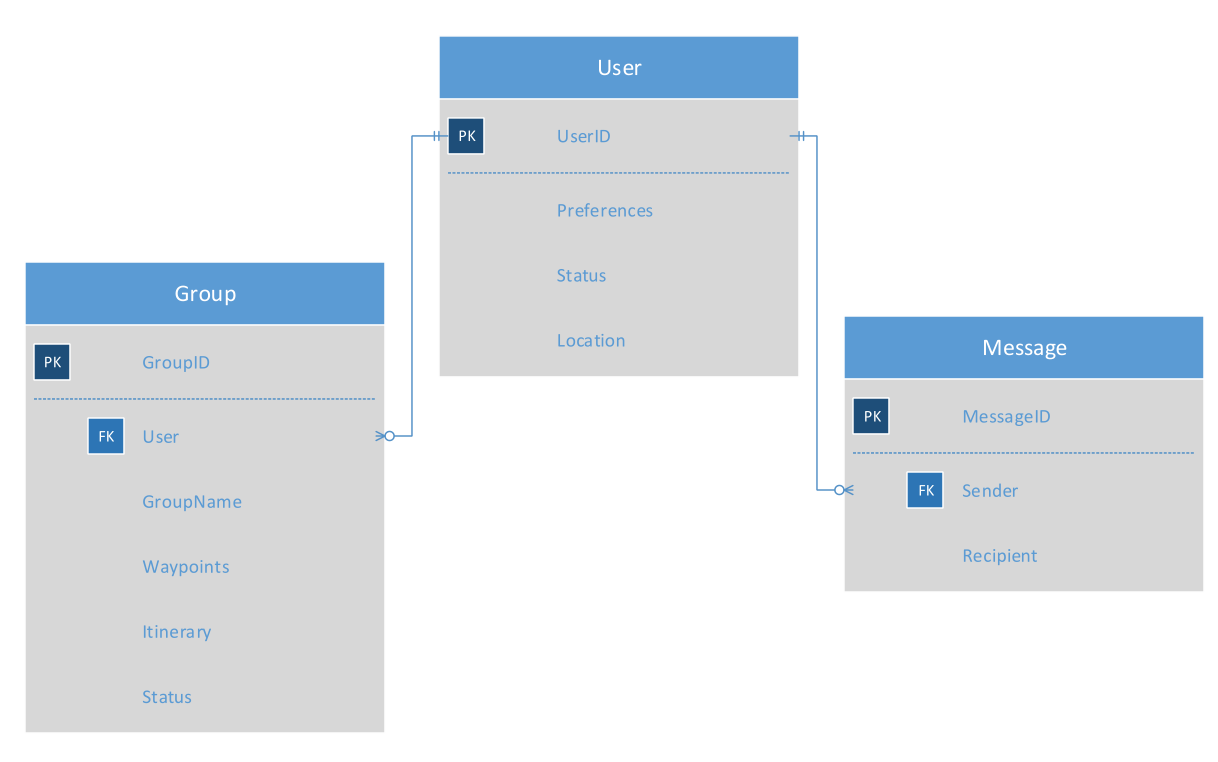
\includegraphics[scale=.6]{Additional/DesignPictures/CC_dbSchema1.PNG}}
	\end{center}
	\caption{Early database schema. \label{EarlyDBSchema}}
	\end{figure}

Another caveat to this design is the failure to differentiate between public and private user data. In Crowd Control, each user has data that is private to that user, such as their email and password. However, there is also a set of public data that can be viewed by other users, such as their display name or their location. This iteration of the schema only has one user entity, that stores their information. A small lack of understanding about Parse's no-SQL implementation lead us to improperly design our entities in this way. It was later deemed that this separation between front-facing and hidden user data entities was necessary in terms of ease-of-access and information privacy.

\subsubsection{Improvements to Early Designs}
In reflection of the shortcomings of the first design iteration, the database schema was restructured to better fit Crowd Control's needs. More entities were added to the overall schema. One such addition was a ``CCUser'' table to hold the public data associated with a user. It is important to note that the ``User'' table was left to hold a user's private data. Those changes and some additions resulted in the below schema. 

	\begin{figure}[tbh]
	\begin{center}
	\fbox{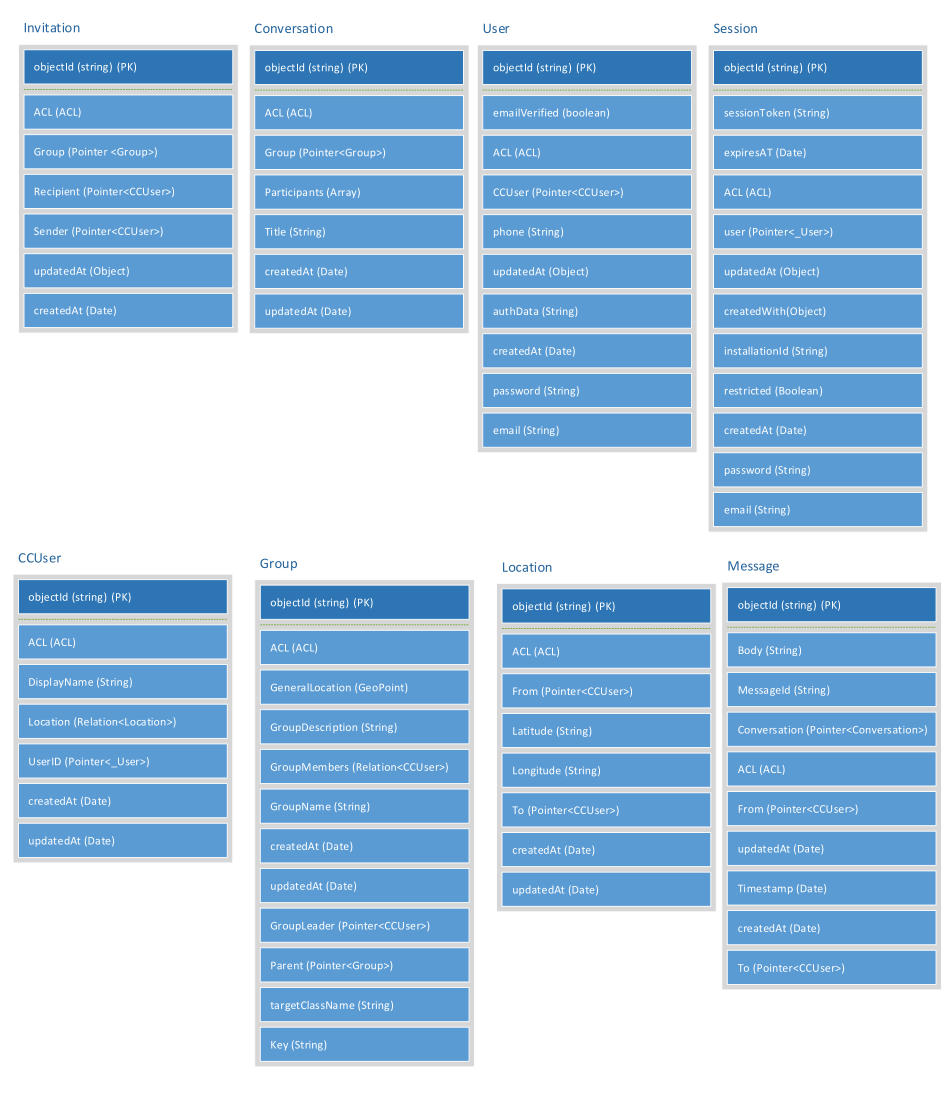
\includegraphics[scale=.6]{Additional/DesignPictures/CC_dbSchema2.PNG}}
	\end{center}
	\caption{Early database schema. \label{EarlyDBSchema}}
	\end{figure}

\subsubsection{Current Design}
(What we have now, further concerns?)
 
 \subsection{Data Structures and Algorithms}
 Describe the special data structures and any special algorithms.
 
 \subsection{Data Flow}
 
 \subsection{Communications}
 
 \subsection{Classes}
 
 \subsection{UML}
 
 \subsection{GUI}
 
 \subsection{MVVM, etc}

\section{Major Component \#1 }

\subsection{Technologies  Used}
This section provides a list of technologies used for this component.  The details 
for the technologies have already been provided in the Overview section. 

\subsection{Component  Overview}
This section can take the form of a list of features. 

\subsection{Phase Overview}
This is an extension of the Phase Overview above, but specific to this component. 
 It is meant to be basically a brief list with space for marking the phase status. 

\subsection{ Architecture  Diagram}
It is important to build and maintain an architecture diagram.  However, it may 
be that a component is best described visually with a data flow diagram. 


\subsection{Data Flow Diagram}
It is important to build and maintain a data flow diagram.  However, it may be 
that a component is best described visually with an architecture diagram. 


\subsection{Design Details}
This is where the details are presented and may contain subsections.   Here is an example code listing:
\begin{lstlisting}
#include <stdio.h>
#define N 10
/* Block
 * comment */
 
int main()
{
    int i;
 
    // Line comment.
    puts("Hello world!");
 
    for (i = 0; i < N; i++)
    {
        puts("LaTeX is also great for programmers!");
    }
 
    return 0;
}
\end{lstlisting}
This code listing is not floating or automatically numbered.  If you want auto-numbering, but it in the algorithm environment (not algorithmic however) shown above.



\section{Major Component \#2 }

\subsection{Technologies  Used}
This section provides a list of technologies used for this component.  The details 
for the technologies have already been provided in the Overview section. 

\subsection{Component  Overview}
This section can take the form of a list of features. 

\subsection{Phase Overview}
This is an extension of the Phase Overview above, but specific to this component. 
 It is meant to be basically a brief list with space for marking the phase status. 

\subsection{ Architecture  Diagram}
It is important to build and maintain an architecture diagram.  However, it may 
be that a component is best described visually with a data flow diagram. 


\subsection{Data Flow Diagram}
It is important to build and maintain a data flow diagram.  However, it may be 
that a component is best described visually with an architecture diagram. 


\subsection{Design Details}
This is where the details are presented and may contain subsections. 


\section{Major Component \#3 }

\subsection{Technologies  Used}
This section provides a list of technologies used for this component.  The details 
for the technologies have already been provided in the Overview section. 

\subsection{Component  Overview}
This section can take the form of a list of features. 

\subsection{Phase Overview}
This is an extension of the Phase Overview above, but specific to this component. 
 It is meant to be basically a brief list with space for marking the phase status. 

\subsection{ Architecture  Diagram}
It is important to build and maintain an architecture diagram.  However, it may 
be that a component is best described visually with a data flow diagram. 


\subsection{Data Flow Diagram}
It is important to build and maintain a data flow diagram.  However, it may be 
that a component is best described visually with an architecture diagram. 


\subsection{Design Details}
This is where the details are presented and may contain subsections. 


